% ---------------------------------------------------------------
% Generated by FlowTikZ (flowcharts and data charts to LaTeX)
% Every coordinate below is derived from the editor diagram model.
% Safe to edit by hand, but regenerating will overwrite changes.
% ---------------------------------------------------------------

\documentclass[border=8pt]{standalone}
\usepackage[T1]{fontenc}
\usepackage[utf8]{inputenc}
\usepackage{amsmath}
\usepackage{xcolor}
\usepackage{tikz}
\usetikzlibrary{arrows.meta,shapes.geometric,shapes.misc}

% ---- Colour definitions ----
\definecolor{fc12161C}{HTML}{12161C}
\definecolor{fc1F2933}{HTML}{1F2933}
\definecolor{fcD4F0EA}{HTML}{D4F0EA}
\definecolor{fcDBE8FF}{HTML}{DBE8FF}
\definecolor{fcDCFCE7}{HTML}{DCFCE7}
\definecolor{fcE0F2FE}{HTML}{E0F2FE}
\definecolor{fcE6EDF4}{HTML}{E6EDF4}
\definecolor{fcE8F0FF}{HTML}{E8F0FF}
\definecolor{fcEEF2FF}{HTML}{EEF2FF}
\definecolor{fcFADFD8}{HTML}{FADFD8}
\definecolor{fcFAE8FF}{HTML}{FAE8FF}
\definecolor{fcFEF9C3}{HTML}{FEF9C3}
\definecolor{fcFFEDD5}{HTML}{FFEDD5}
\definecolor{fcFFF4D6}{HTML}{FFF4D6}

% ---- Style definitions ----
\tikzset{
  fcnode/.style={
    draw, inner sep=0pt, outer sep=0pt, align=center,
    line join=round, line cap=butt
  },
  fcpath/.style={line join=round, line cap=butt},
  fcedge/.style={line join=round, line cap=butt},
  fclabel/.style={inner sep=1.4pt, outer sep=0pt, align=center},
}

\begin{document}
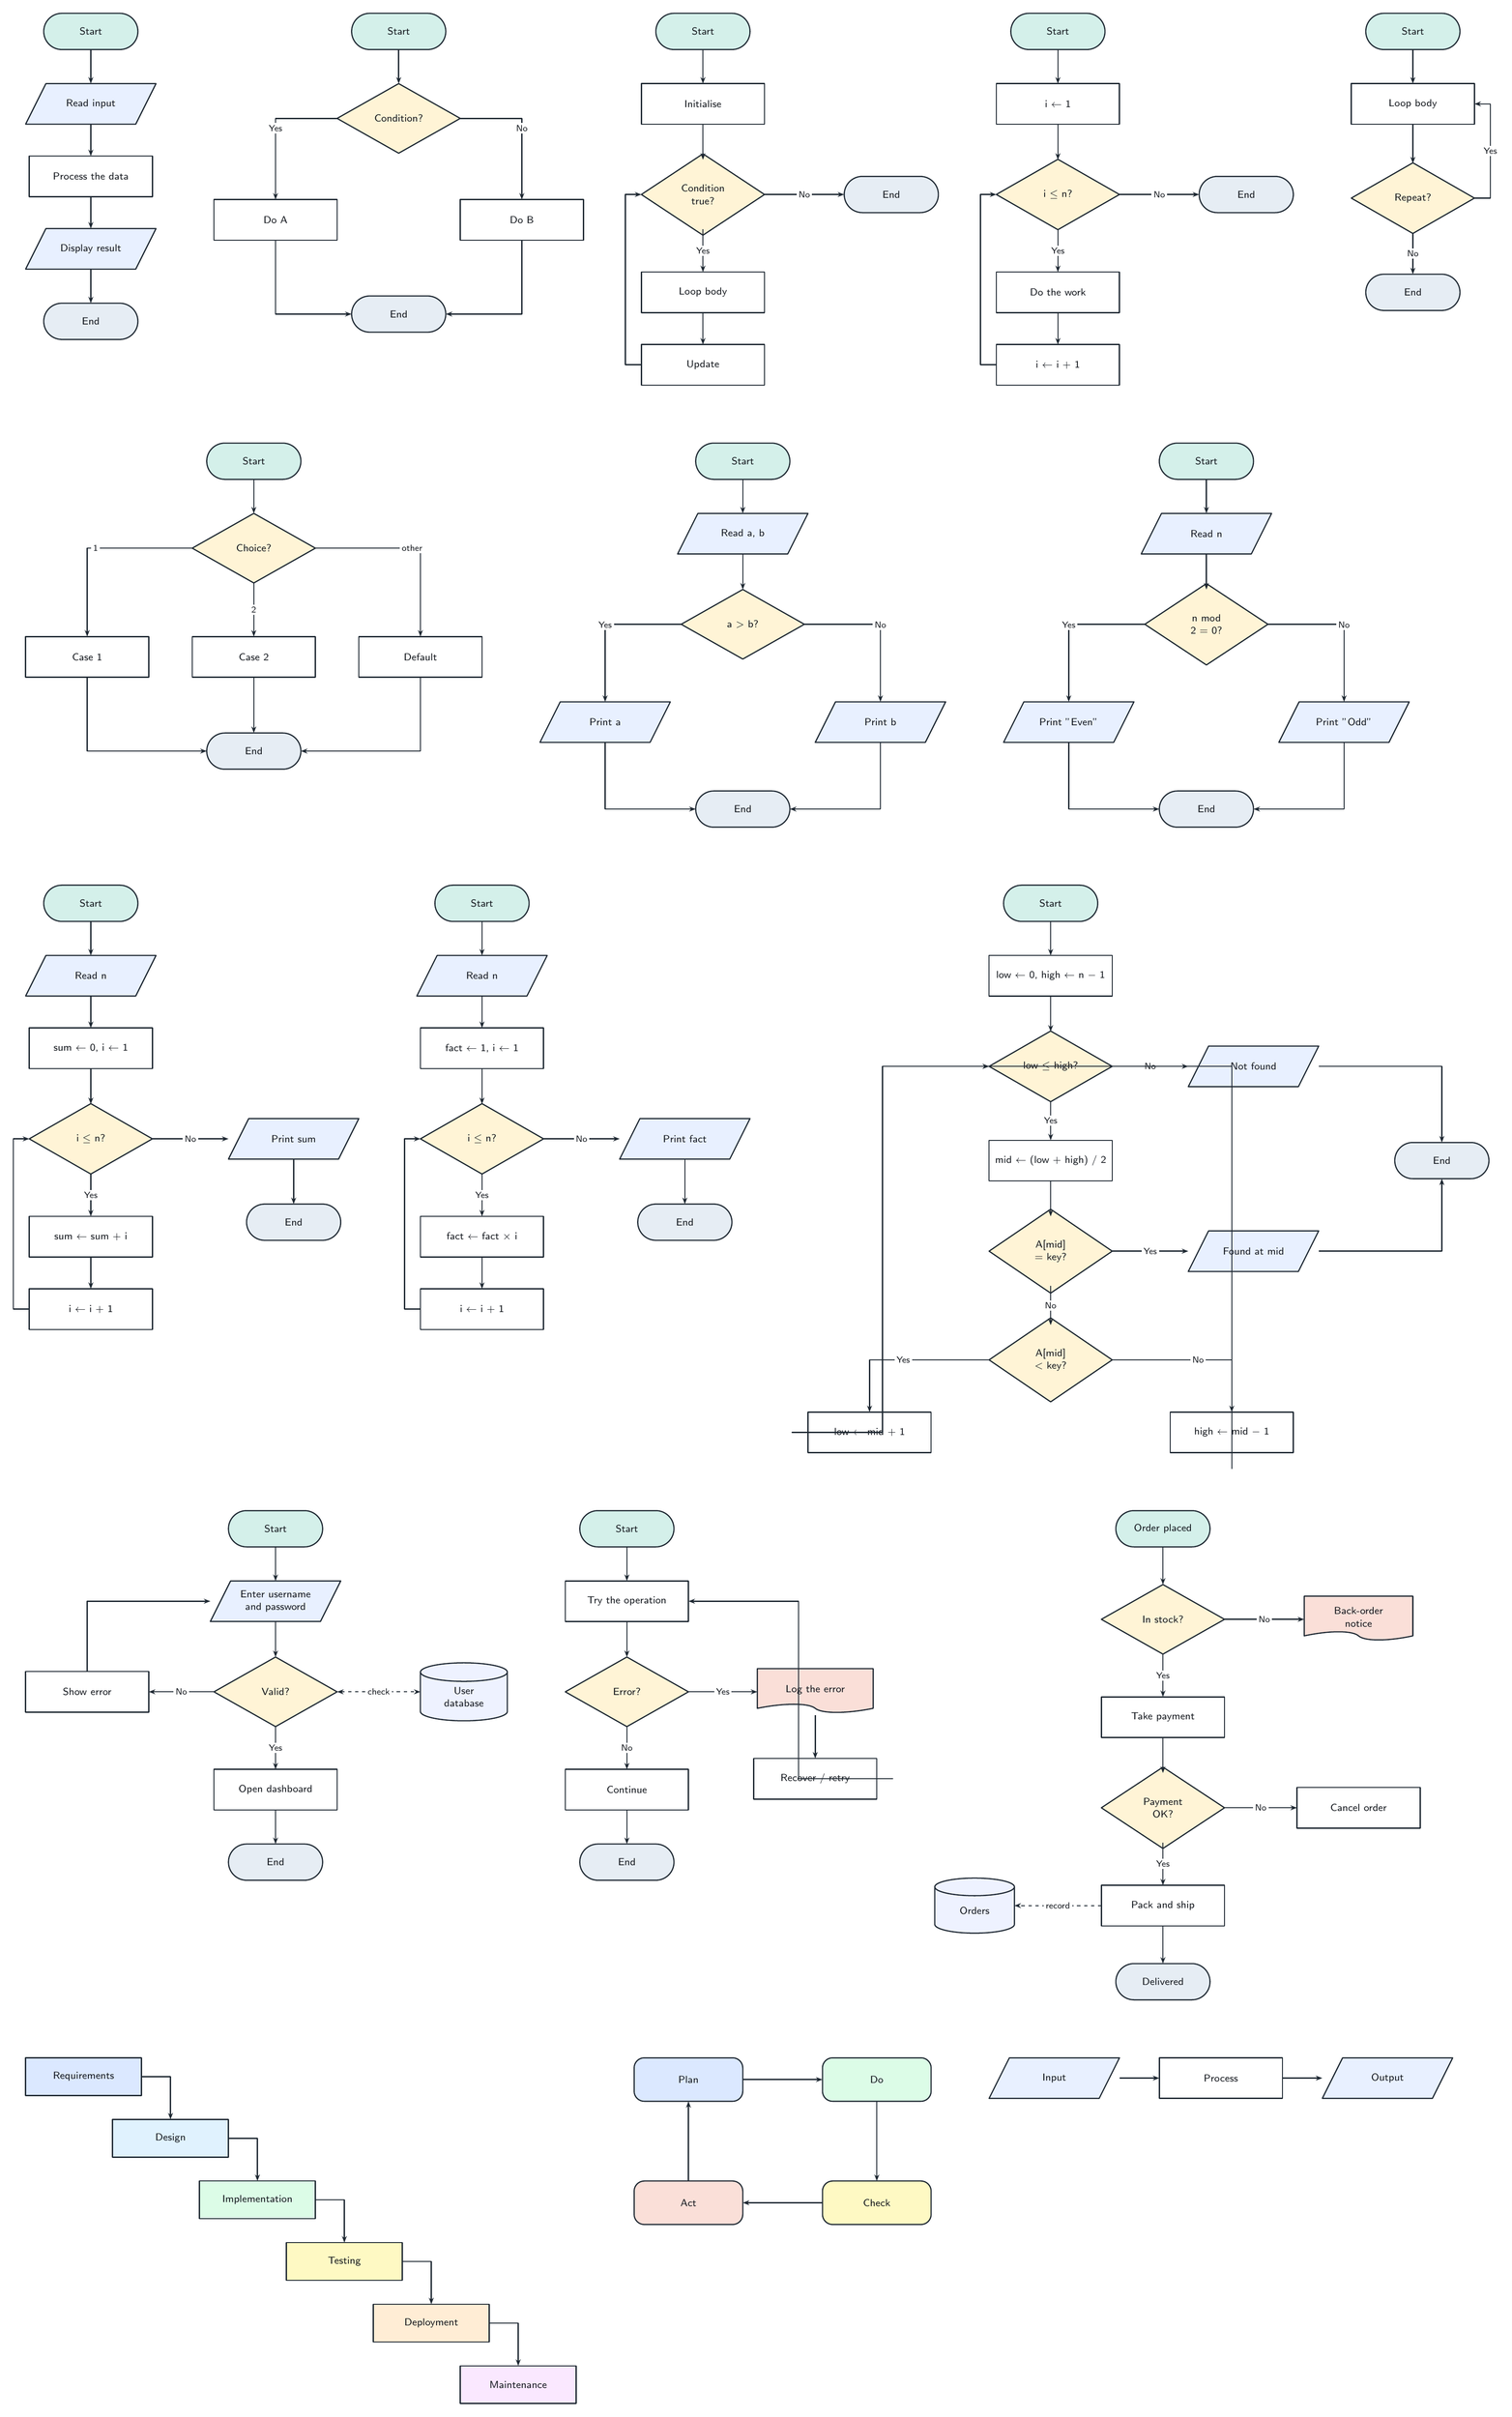
\begin{tikzpicture}[x=1cm, y=1cm]
  % ---- Nodes ----
  % g1 - Start / End "Start"
  \node[fcnode, shape=rounded rectangle, minimum width=2.6cm, minimum height=1cm,
        rounded rectangle arc length=180, draw=fc1F2933, line width=0.91pt, fill=fcD4F0EA,
        font=\fontsize{7.97pt}{9.96pt}\selectfont\sffamily, text=fc12161C, align=center,
        text width=2cm] (g1) at (3.8,-2.5) {Start};
  % g2 - Input / Output "Read input"
  \draw[fcpath, draw=fc1F2933, line width=0.91pt, fill=fcE8F0FF]
    (2.56,-3.94) -- (5.6,-3.94) -- (5.04,-5.06) -- (2,-5.06) -- cycle;
  \coordinate (g2) at (3.8,-4.5);
  \node[fclabel, anchor=center, font=\fontsize{7.97pt}{9.96pt}\selectfont\sffamily,
        text=fc12161C, align=center, text width=2.368cm] at (3.8,-4.5) {Read input};
  % g3 - Process "Process the data"
  \node[fcnode, shape=rectangle, minimum width=3.4cm, minimum height=1.12cm, draw=fc1F2933,
        line width=0.91pt, fill=white, font=\fontsize{7.97pt}{9.96pt}\selectfont\sffamily,
        text=fc12161C, align=center, text width=3.08cm] (g3) at (3.8,-6.5) {Process the data};
  % g4 - Input / Output "Display result"
  \draw[fcpath, draw=fc1F2933, line width=0.91pt, fill=fcE8F0FF]
    (2.56,-7.94) -- (5.6,-7.94) -- (5.04,-9.06) -- (2,-9.06) -- cycle;
  \coordinate (g4) at (3.8,-8.5);
  \node[fclabel, anchor=center, font=\fontsize{7.97pt}{9.96pt}\selectfont\sffamily,
        text=fc12161C, align=center, text width=2.368cm] at (3.8,-8.5) {Display result};
  % g5 - Start / End "End"
  \node[fcnode, shape=rounded rectangle, minimum width=2.6cm, minimum height=1cm,
        rounded rectangle arc length=180, draw=fc1F2933, line width=0.91pt, fill=fcE6EDF4,
        font=\fontsize{7.97pt}{9.96pt}\selectfont\sffamily, text=fc12161C, align=center,
        text width=2cm] (g5) at (3.8,-10.5) {End};
  % g10 - Start / End "Start"
  \node[fcnode, shape=rounded rectangle, minimum width=2.6cm, minimum height=1cm,
        rounded rectangle arc length=180, draw=fc1F2933, line width=0.91pt, fill=fcD4F0EA,
        font=\fontsize{7.97pt}{9.96pt}\selectfont\sffamily, text=fc12161C, align=center,
        text width=2cm] (g10) at (12.3,-2.5) {Start};
  % g11 - Decision "Condition?"
  \node[fcnode, shape=diamond, minimum width=3.4cm, minimum height=1.92cm, draw=fc1F2933,
        line width=0.91pt, fill=fcFFF4D6, font=\fontsize{7.97pt}{9.96pt}\selectfont\sffamily,
        text=fc12161C, align=center, text width=1.7cm] (g11) at (12.3,-4.9) {Condition?};
  % g12 - Process "Do A"
  \node[fcnode, shape=rectangle, minimum width=3.4cm, minimum height=1.12cm, draw=fc1F2933,
        line width=0.91pt, fill=white, font=\fontsize{7.97pt}{9.96pt}\selectfont\sffamily,
        text=fc12161C, align=center, text width=3.08cm] (g12) at (8.9,-7.7) {Do A};
  % g13 - Process "Do B"
  \node[fcnode, shape=rectangle, minimum width=3.4cm, minimum height=1.12cm, draw=fc1F2933,
        line width=0.91pt, fill=white, font=\fontsize{7.97pt}{9.96pt}\selectfont\sffamily,
        text=fc12161C, align=center, text width=3.08cm] (g13) at (15.7,-7.7) {Do B};
  % g14 - Start / End "End"
  \node[fcnode, shape=rounded rectangle, minimum width=2.6cm, minimum height=1cm,
        rounded rectangle arc length=180, draw=fc1F2933, line width=0.91pt, fill=fcE6EDF4,
        font=\fontsize{7.97pt}{9.96pt}\selectfont\sffamily, text=fc12161C, align=center,
        text width=2cm] (g14) at (12.3,-10.3) {End};
  % g20 - Start / End "Start"
  \node[fcnode, shape=rounded rectangle, minimum width=2.6cm, minimum height=1cm,
        rounded rectangle arc length=180, draw=fc1F2933, line width=0.91pt, fill=fcD4F0EA,
        font=\fontsize{7.97pt}{9.96pt}\selectfont\sffamily, text=fc12161C, align=center,
        text width=2cm] (g20) at (20.7,-2.5) {Start};
  % g21 - Process "Initialise"
  \node[fcnode, shape=rectangle, minimum width=3.4cm, minimum height=1.12cm, draw=fc1F2933,
        line width=0.91pt, fill=white, font=\fontsize{7.97pt}{9.96pt}\selectfont\sffamily,
        text=fc12161C, align=center, text width=3.08cm] (g21) at (20.7,-4.5) {Initialise};
  % g22 - Decision "Condition"
  \node[fcnode, shape=diamond, minimum width=3.4cm, minimum height=1.92cm, draw=fc1F2933,
        line width=0.91pt, fill=fcFFF4D6, font=\fontsize{7.97pt}{9.96pt}\selectfont\sffamily,
        text=fc12161C, align=center, text width=1.7cm]
        (g22) at (20.7,-7) {Condition \\ true?};
  % g23 - Process "Loop body"
  \node[fcnode, shape=rectangle, minimum width=3.4cm, minimum height=1.12cm, draw=fc1F2933,
        line width=0.91pt, fill=white, font=\fontsize{7.97pt}{9.96pt}\selectfont\sffamily,
        text=fc12161C, align=center, text width=3.08cm] (g23) at (20.7,-9.7) {Loop body};
  % g24 - Process "Update"
  \node[fcnode, shape=rectangle, minimum width=3.4cm, minimum height=1.12cm, draw=fc1F2933,
        line width=0.91pt, fill=white, font=\fontsize{7.97pt}{9.96pt}\selectfont\sffamily,
        text=fc12161C, align=center, text width=3.08cm] (g24) at (20.7,-11.7) {Update};
  % g25 - Start / End "End"
  \node[fcnode, shape=rounded rectangle, minimum width=2.6cm, minimum height=1cm,
        rounded rectangle arc length=180, draw=fc1F2933, line width=0.91pt, fill=fcE6EDF4,
        font=\fontsize{7.97pt}{9.96pt}\selectfont\sffamily, text=fc12161C, align=center,
        text width=2cm] (g25) at (25.9,-7) {End};
  % g32 - Start / End "Start"
  \node[fcnode, shape=rounded rectangle, minimum width=2.6cm, minimum height=1cm,
        rounded rectangle arc length=180, draw=fc1F2933, line width=0.91pt, fill=fcD4F0EA,
        font=\fontsize{7.97pt}{9.96pt}\selectfont\sffamily, text=fc12161C, align=center,
        text width=2cm] (g32) at (30.5,-2.5) {Start};
  % g33 - Process "i ← 1"
  \node[fcnode, shape=rectangle, minimum width=3.4cm, minimum height=1.12cm, draw=fc1F2933,
        line width=0.91pt, fill=white, font=\fontsize{7.97pt}{9.96pt}\selectfont\sffamily,
        text=fc12161C, align=center, text width=3.08cm]
        (g33) at (30.5,-4.5) {i $\leftarrow$ 1};
  % g34 - Decision "i ≤ n?"
  \node[fcnode, shape=diamond, minimum width=3.4cm, minimum height=1.92cm, draw=fc1F2933,
        line width=0.91pt, fill=fcFFF4D6, font=\fontsize{7.97pt}{9.96pt}\selectfont\sffamily,
        text=fc12161C, align=center, text width=1.7cm] (g34) at (30.5,-7) {i $\leq$ n?};
  % g35 - Process "Do the work"
  \node[fcnode, shape=rectangle, minimum width=3.4cm, minimum height=1.12cm, draw=fc1F2933,
        line width=0.91pt, fill=white, font=\fontsize{7.97pt}{9.96pt}\selectfont\sffamily,
        text=fc12161C, align=center, text width=3.08cm] (g35) at (30.5,-9.7) {Do the work};
  % g36 - Process "i ← i + 1"
  \node[fcnode, shape=rectangle, minimum width=3.4cm, minimum height=1.12cm, draw=fc1F2933,
        line width=0.91pt, fill=white, font=\fontsize{7.97pt}{9.96pt}\selectfont\sffamily,
        text=fc12161C, align=center, text width=3.08cm]
        (g36) at (30.5,-11.7) {i $\leftarrow$ i + 1};
  % g37 - Start / End "End"
  \node[fcnode, shape=rounded rectangle, minimum width=2.6cm, minimum height=1cm,
        rounded rectangle arc length=180, draw=fc1F2933, line width=0.91pt, fill=fcE6EDF4,
        font=\fontsize{7.97pt}{9.96pt}\selectfont\sffamily, text=fc12161C, align=center,
        text width=2cm] (g37) at (35.7,-7) {End};
  % g44 - Start / End "Start"
  \node[fcnode, shape=rounded rectangle, minimum width=2.6cm, minimum height=1cm,
        rounded rectangle arc length=180, draw=fc1F2933, line width=0.91pt, fill=fcD4F0EA,
        font=\fontsize{7.97pt}{9.96pt}\selectfont\sffamily, text=fc12161C, align=center,
        text width=2cm] (g44) at (40.3,-2.5) {Start};
  % g45 - Process "Loop body"
  \node[fcnode, shape=rectangle, minimum width=3.4cm, minimum height=1.12cm, draw=fc1F2933,
        line width=0.91pt, fill=white, font=\fontsize{7.97pt}{9.96pt}\selectfont\sffamily,
        text=fc12161C, align=center, text width=3.08cm] (g45) at (40.3,-4.5) {Loop body};
  % g46 - Decision "Repeat?"
  \node[fcnode, shape=diamond, minimum width=3.4cm, minimum height=1.92cm, draw=fc1F2933,
        line width=0.91pt, fill=fcFFF4D6, font=\fontsize{7.97pt}{9.96pt}\selectfont\sffamily,
        text=fc12161C, align=center, text width=1.7cm] (g46) at (40.3,-7.1) {Repeat?};
  % g47 - Start / End "End"
  \node[fcnode, shape=rounded rectangle, minimum width=2.6cm, minimum height=1cm,
        rounded rectangle arc length=180, draw=fc1F2933, line width=0.91pt, fill=fcE6EDF4,
        font=\fontsize{7.97pt}{9.96pt}\selectfont\sffamily, text=fc12161C, align=center,
        text width=2cm] (g47) at (40.3,-9.7) {End};
  % g52 - Start / End "Start"
  \node[fcnode, shape=rounded rectangle, minimum width=2.6cm, minimum height=1cm,
        rounded rectangle arc length=180, draw=fc1F2933, line width=0.91pt, fill=fcD4F0EA,
        font=\fontsize{7.97pt}{9.96pt}\selectfont\sffamily, text=fc12161C, align=center,
        text width=2cm] (g52) at (8.3,-14.36) {Start};
  % g53 - Decision "Choice?"
  \node[fcnode, shape=diamond, minimum width=3.4cm, minimum height=1.92cm, draw=fc1F2933,
        line width=0.91pt, fill=fcFFF4D6, font=\fontsize{7.97pt}{9.96pt}\selectfont\sffamily,
        text=fc12161C, align=center, text width=1.7cm] (g53) at (8.3,-16.76) {Choice?};
  % g54 - Process "Case 1"
  \node[fcnode, shape=rectangle, minimum width=3.4cm, minimum height=1.12cm, draw=fc1F2933,
        line width=0.91pt, fill=white, font=\fontsize{7.97pt}{9.96pt}\selectfont\sffamily,
        text=fc12161C, align=center, text width=3.08cm] (g54) at (3.7,-19.76) {Case 1};
  % g55 - Process "Case 2"
  \node[fcnode, shape=rectangle, minimum width=3.4cm, minimum height=1.12cm, draw=fc1F2933,
        line width=0.91pt, fill=white, font=\fontsize{7.97pt}{9.96pt}\selectfont\sffamily,
        text=fc12161C, align=center, text width=3.08cm] (g55) at (8.3,-19.76) {Case 2};
  % g56 - Process "Default"
  \node[fcnode, shape=rectangle, minimum width=3.4cm, minimum height=1.12cm, draw=fc1F2933,
        line width=0.91pt, fill=white, font=\fontsize{7.97pt}{9.96pt}\selectfont\sffamily,
        text=fc12161C, align=center, text width=3.08cm] (g56) at (12.9,-19.76) {Default};
  % g57 - Start / End "End"
  \node[fcnode, shape=rounded rectangle, minimum width=2.6cm, minimum height=1cm,
        rounded rectangle arc length=180, draw=fc1F2933, line width=0.91pt, fill=fcE6EDF4,
        font=\fontsize{7.97pt}{9.96pt}\selectfont\sffamily, text=fc12161C, align=center,
        text width=2cm] (g57) at (8.3,-22.36) {End};
  % g65 - Start / End "Start"
  \node[fcnode, shape=rounded rectangle, minimum width=2.6cm, minimum height=1cm,
        rounded rectangle arc length=180, draw=fc1F2933, line width=0.91pt, fill=fcD4F0EA,
        font=\fontsize{7.97pt}{9.96pt}\selectfont\sffamily, text=fc12161C, align=center,
        text width=2cm] (g65) at (21.8,-14.36) {Start};
  % g66 - Input / Output "Read a, b"
  \draw[fcpath, draw=fc1F2933, line width=0.91pt, fill=fcE8F0FF]
    (20.56,-15.8) -- (23.6,-15.8) -- (23.04,-16.92) -- (20,-16.92) -- cycle;
  \coordinate (g66) at (21.8,-16.36);
  \node[fclabel, anchor=center, font=\fontsize{7.97pt}{9.96pt}\selectfont\sffamily,
        text=fc12161C, align=center, text width=2.368cm] at (21.8,-16.36) {Read a, b};
  % g67 - Decision "a > b?"
  \node[fcnode, shape=diamond, minimum width=3.4cm, minimum height=1.92cm, draw=fc1F2933,
        line width=0.91pt, fill=fcFFF4D6, font=\fontsize{7.97pt}{9.96pt}\selectfont\sffamily,
        text=fc12161C, align=center, text width=1.7cm]
        (g67) at (21.8,-18.86) {a \textgreater{} b?};
  % g68 - Input / Output "Print a"
  \draw[fcpath, draw=fc1F2933, line width=0.91pt, fill=fcE8F0FF]
    (16.76,-21) -- (19.8,-21) -- (19.24,-22.12) -- (16.2,-22.12) -- cycle;
  \coordinate (g68) at (18,-21.56);
  \node[fclabel, anchor=center, font=\fontsize{7.97pt}{9.96pt}\selectfont\sffamily,
        text=fc12161C, align=center, text width=2.368cm] at (18,-21.56) {Print a};
  % g69 - Input / Output "Print b"
  \draw[fcpath, draw=fc1F2933, line width=0.91pt, fill=fcE8F0FF]
    (24.36,-21) -- (27.4,-21) -- (26.84,-22.12) -- (23.8,-22.12) -- cycle;
  \coordinate (g69) at (25.6,-21.56);
  \node[fclabel, anchor=center, font=\fontsize{7.97pt}{9.96pt}\selectfont\sffamily,
        text=fc12161C, align=center, text width=2.368cm] at (25.6,-21.56) {Print b};
  % g70 - Start / End "End"
  \node[fcnode, shape=rounded rectangle, minimum width=2.6cm, minimum height=1cm,
        rounded rectangle arc length=180, draw=fc1F2933, line width=0.91pt, fill=fcE6EDF4,
        font=\fontsize{7.97pt}{9.96pt}\selectfont\sffamily, text=fc12161C, align=center,
        text width=2cm] (g70) at (21.8,-23.96) {End};
  % g77 - Start / End "Start"
  \node[fcnode, shape=rounded rectangle, minimum width=2.6cm, minimum height=1cm,
        rounded rectangle arc length=180, draw=fc1F2933, line width=0.91pt, fill=fcD4F0EA,
        font=\fontsize{7.97pt}{9.96pt}\selectfont\sffamily, text=fc12161C, align=center,
        text width=2cm] (g77) at (34.6,-14.36) {Start};
  % g78 - Input / Output "Read n"
  \draw[fcpath, draw=fc1F2933, line width=0.91pt, fill=fcE8F0FF]
    (33.36,-15.8) -- (36.4,-15.8) -- (35.84,-16.92) -- (32.8,-16.92) -- cycle;
  \coordinate (g78) at (34.6,-16.36);
  \node[fclabel, anchor=center, font=\fontsize{7.97pt}{9.96pt}\selectfont\sffamily,
        text=fc12161C, align=center, text width=2.368cm] at (34.6,-16.36) {Read n};
  % g79 - Decision "n mod 2 = 0?"
  \node[fcnode, shape=diamond, minimum width=3.4cm, minimum height=1.92cm, draw=fc1F2933,
        line width=0.91pt, fill=fcFFF4D6, font=\fontsize{7.97pt}{9.96pt}\selectfont\sffamily,
        text=fc12161C, align=center, text width=1.7cm] (g79) at (34.6,-18.86) {n mod 2 = 0?};
  % g80 - Input / Output "Print "Even""
  \draw[fcpath, draw=fc1F2933, line width=0.91pt, fill=fcE8F0FF]
    (29.56,-21) -- (32.6,-21) -- (32.04,-22.12) -- (29,-22.12) -- cycle;
  \coordinate (g80) at (30.8,-21.56);
  \node[fclabel, anchor=center, font=\fontsize{7.97pt}{9.96pt}\selectfont\sffamily,
        text=fc12161C, align=center, text width=2.368cm] at (30.8,-21.56) {Print "Even"};
  % g81 - Input / Output "Print "Odd""
  \draw[fcpath, draw=fc1F2933, line width=0.91pt, fill=fcE8F0FF]
    (37.16,-21) -- (40.2,-21) -- (39.64,-22.12) -- (36.6,-22.12) -- cycle;
  \coordinate (g81) at (38.4,-21.56);
  \node[fclabel, anchor=center, font=\fontsize{7.97pt}{9.96pt}\selectfont\sffamily,
        text=fc12161C, align=center, text width=2.368cm] at (38.4,-21.56) {Print "Odd"};
  % g82 - Start / End "End"
  \node[fcnode, shape=rounded rectangle, minimum width=2.6cm, minimum height=1cm,
        rounded rectangle arc length=180, draw=fc1F2933, line width=0.91pt, fill=fcE6EDF4,
        font=\fontsize{7.97pt}{9.96pt}\selectfont\sffamily, text=fc12161C, align=center,
        text width=2cm] (g82) at (34.6,-23.96) {End};
  % g89 - Start / End "Start"
  \node[fcnode, shape=rounded rectangle, minimum width=2.6cm, minimum height=1cm,
        rounded rectangle arc length=180, draw=fc1F2933, line width=0.91pt, fill=fcD4F0EA,
        font=\fontsize{7.97pt}{9.96pt}\selectfont\sffamily, text=fc12161C, align=center,
        text width=2cm] (g89) at (3.8,-26.56) {Start};
  % g90 - Input / Output "Read n"
  \draw[fcpath, draw=fc1F2933, line width=0.91pt, fill=fcE8F0FF]
    (2.56,-28) -- (5.6,-28) -- (5.04,-29.12) -- (2,-29.12) -- cycle;
  \coordinate (g90) at (3.8,-28.56);
  \node[fclabel, anchor=center, font=\fontsize{7.97pt}{9.96pt}\selectfont\sffamily,
        text=fc12161C, align=center, text width=2.368cm] at (3.8,-28.56) {Read n};
  % g91 - Process "sum ← 0, i ← 1"
  \node[fcnode, shape=rectangle, minimum width=3.4cm, minimum height=1.12cm, draw=fc1F2933,
        line width=0.91pt, fill=white, font=\fontsize{7.97pt}{9.96pt}\selectfont\sffamily,
        text=fc12161C, align=center, text width=3.08cm]
        (g91) at (3.8,-30.56) {sum $\leftarrow$ 0, i $\leftarrow$ 1};
  % g92 - Decision "i ≤ n?"
  \node[fcnode, shape=diamond, minimum width=3.4cm, minimum height=1.92cm, draw=fc1F2933,
        line width=0.91pt, fill=fcFFF4D6, font=\fontsize{7.97pt}{9.96pt}\selectfont\sffamily,
        text=fc12161C, align=center, text width=1.7cm] (g92) at (3.8,-33.06) {i $\leq$ n?};
  % g93 - Process "sum ← sum + i"
  \node[fcnode, shape=rectangle, minimum width=3.4cm, minimum height=1.12cm, draw=fc1F2933,
        line width=0.91pt, fill=white, font=\fontsize{7.97pt}{9.96pt}\selectfont\sffamily,
        text=fc12161C, align=center, text width=3.08cm]
        (g93) at (3.8,-35.76) {sum $\leftarrow$ sum + i};
  % g94 - Process "i ← i + 1"
  \node[fcnode, shape=rectangle, minimum width=3.4cm, minimum height=1.12cm, draw=fc1F2933,
        line width=0.91pt, fill=white, font=\fontsize{7.97pt}{9.96pt}\selectfont\sffamily,
        text=fc12161C, align=center, text width=3.08cm]
        (g94) at (3.8,-37.76) {i $\leftarrow$ i + 1};
  % g95 - Input / Output "Print sum"
  \draw[fcpath, draw=fc1F2933, line width=0.91pt, fill=fcE8F0FF]
    (8.16,-32.5) -- (11.2,-32.5) -- (10.64,-33.62) -- (7.6,-33.62) -- cycle;
  \coordinate (g95) at (9.4,-33.06);
  \node[fclabel, anchor=center, font=\fontsize{7.97pt}{9.96pt}\selectfont\sffamily,
        text=fc12161C, align=center, text width=2.368cm] at (9.4,-33.06) {Print sum};
  % g96 - Start / End "End"
  \node[fcnode, shape=rounded rectangle, minimum width=2.6cm, minimum height=1cm,
        rounded rectangle arc length=180, draw=fc1F2933, line width=0.91pt, fill=fcE6EDF4,
        font=\fontsize{7.97pt}{9.96pt}\selectfont\sffamily, text=fc12161C, align=center,
        text width=2cm] (g96) at (9.4,-35.36) {End};
  % g105 - Start / End "Start"
  \node[fcnode, shape=rounded rectangle, minimum width=2.6cm, minimum height=1cm,
        rounded rectangle arc length=180, draw=fc1F2933, line width=0.91pt, fill=fcD4F0EA,
        font=\fontsize{7.97pt}{9.96pt}\selectfont\sffamily, text=fc12161C, align=center,
        text width=2cm] (g105) at (14.6,-26.56) {Start};
  % g106 - Input / Output "Read n"
  \draw[fcpath, draw=fc1F2933, line width=0.91pt, fill=fcE8F0FF]
    (13.36,-28) -- (16.4,-28) -- (15.84,-29.12) -- (12.8,-29.12) -- cycle;
  \coordinate (g106) at (14.6,-28.56);
  \node[fclabel, anchor=center, font=\fontsize{7.97pt}{9.96pt}\selectfont\sffamily,
        text=fc12161C, align=center, text width=2.368cm] at (14.6,-28.56) {Read n};
  % g107 - Process "fact ← 1, i ← 1"
  \node[fcnode, shape=rectangle, minimum width=3.4cm, minimum height=1.12cm, draw=fc1F2933,
        line width=0.91pt, fill=white, font=\fontsize{7.97pt}{9.96pt}\selectfont\sffamily,
        text=fc12161C, align=center, text width=3.08cm]
        (g107) at (14.6,-30.56) {fact $\leftarrow$ 1, i $\leftarrow$ 1};
  % g108 - Decision "i ≤ n?"
  \node[fcnode, shape=diamond, minimum width=3.4cm, minimum height=1.92cm, draw=fc1F2933,
        line width=0.91pt, fill=fcFFF4D6, font=\fontsize{7.97pt}{9.96pt}\selectfont\sffamily,
        text=fc12161C, align=center, text width=1.7cm] (g108) at (14.6,-33.06) {i $\leq$ n?};
  % g109 - Process "fact ← fact × i"
  \node[fcnode, shape=rectangle, minimum width=3.4cm, minimum height=1.12cm, draw=fc1F2933,
        line width=0.91pt, fill=white, font=\fontsize{7.97pt}{9.96pt}\selectfont\sffamily,
        text=fc12161C, align=center, text width=3.08cm]
        (g109) at (14.6,-35.76) {fact $\leftarrow$ fact $\times$ i};
  % g110 - Process "i ← i + 1"
  \node[fcnode, shape=rectangle, minimum width=3.4cm, minimum height=1.12cm, draw=fc1F2933,
        line width=0.91pt, fill=white, font=\fontsize{7.97pt}{9.96pt}\selectfont\sffamily,
        text=fc12161C, align=center, text width=3.08cm]
        (g110) at (14.6,-37.76) {i $\leftarrow$ i + 1};
  % g111 - Input / Output "Print fact"
  \draw[fcpath, draw=fc1F2933, line width=0.91pt, fill=fcE8F0FF]
    (18.96,-32.5) -- (22,-32.5) -- (21.44,-33.62) -- (18.4,-33.62) -- cycle;
  \coordinate (g111) at (20.2,-33.06);
  \node[fclabel, anchor=center, font=\fontsize{7.97pt}{9.96pt}\selectfont\sffamily,
        text=fc12161C, align=center, text width=2.368cm] at (20.2,-33.06) {Print fact};
  % g112 - Start / End "End"
  \node[fcnode, shape=rounded rectangle, minimum width=2.6cm, minimum height=1cm,
        rounded rectangle arc length=180, draw=fc1F2933, line width=0.91pt, fill=fcE6EDF4,
        font=\fontsize{7.97pt}{9.96pt}\selectfont\sffamily, text=fc12161C, align=center,
        text width=2cm] (g112) at (20.2,-35.36) {End};
  % g121 - Start / End "Start"
  \node[fcnode, shape=rounded rectangle, minimum width=2.6cm, minimum height=1cm,
        rounded rectangle arc length=180, draw=fc1F2933, line width=0.91pt, fill=fcD4F0EA,
        font=\fontsize{7.97pt}{9.96pt}\selectfont\sffamily, text=fc12161C, align=center,
        text width=2cm] (g121) at (30.3,-26.56) {Start};
  % g122 - Process "low ← 0, high ← n − 1"
  \node[fcnode, shape=rectangle, minimum width=3.4cm, minimum height=1.12cm, draw=fc1F2933,
        line width=0.91pt, fill=white, font=\fontsize{7.97pt}{9.96pt}\selectfont\sffamily,
        text=fc12161C, align=center, text width=3.08cm]
        (g122) at (30.3,-28.56) {low $\leftarrow$ 0, high $\leftarrow$ n $-$ 1};
  % g123 - Decision "low ≤ high?"
  \node[fcnode, shape=diamond, minimum width=3.4cm, minimum height=1.92cm, draw=fc1F2933,
        line width=0.91pt, fill=fcFFF4D6, font=\fontsize{7.97pt}{9.96pt}\selectfont\sffamily,
        text=fc12161C, align=center, text width=1.7cm]
        (g123) at (30.3,-31.06) {low $\leq$ high?};
  % g124 - Process "mid ← (low + high) / 2"
  \node[fcnode, shape=rectangle, minimum width=3.4cm, minimum height=1.12cm, draw=fc1F2933,
        line width=0.91pt, fill=white, font=\fontsize{7.97pt}{9.96pt}\selectfont\sffamily,
        text=fc12161C, align=center, text width=3.08cm]
        (g124) at (30.3,-33.66) {mid $\leftarrow$ (low + high) / 2};
  % g125 - Decision "A[mid] = key?"
  \node[fcnode, shape=diamond, minimum width=3.4cm, minimum height=1.92cm, draw=fc1F2933,
        line width=0.91pt, fill=fcFFF4D6, font=\fontsize{7.97pt}{9.96pt}\selectfont\sffamily,
        text=fc12161C, align=center, text width=1.7cm]
        (g125) at (30.3,-36.16) {A[mid] = key?};
  % g126 - Input / Output "Found at mid"
  \draw[fcpath, draw=fc1F2933, line width=0.91pt, fill=fcE8F0FF]
    (34.66,-35.6) -- (37.7,-35.6) -- (37.14,-36.72) -- (34.1,-36.72) -- cycle;
  \coordinate (g126) at (35.9,-36.16);
  \node[fclabel, anchor=center, font=\fontsize{7.97pt}{9.96pt}\selectfont\sffamily,
        text=fc12161C, align=center, text width=2.368cm] at (35.9,-36.16) {Found at mid};
  % g127 - Decision "A[mid] < key?"
  \node[fcnode, shape=diamond, minimum width=3.4cm, minimum height=1.92cm, draw=fc1F2933,
        line width=0.91pt, fill=fcFFF4D6, font=\fontsize{7.97pt}{9.96pt}\selectfont\sffamily,
        text=fc12161C, align=center, text width=1.7cm]
        (g127) at (30.3,-39.16) {A[mid] \textless{} key?};
  % g128 - Process "low ← mid + 1"
  \node[fcnode, shape=rectangle, minimum width=3.4cm, minimum height=1.12cm, draw=fc1F2933,
        line width=0.91pt, fill=white, font=\fontsize{7.97pt}{9.96pt}\selectfont\sffamily,
        text=fc12161C, align=center, text width=3.08cm]
        (g128) at (25.3,-41.16) {low $\leftarrow$ mid + 1};
  % g129 - Process "high ← mid − 1"
  \node[fcnode, shape=rectangle, minimum width=3.4cm, minimum height=1.12cm, draw=fc1F2933,
        line width=0.91pt, fill=white, font=\fontsize{7.97pt}{9.96pt}\selectfont\sffamily,
        text=fc12161C, align=center, text width=3.08cm]
        (g129) at (35.3,-41.16) {high $\leftarrow$ mid $-$ 1};
  % g130 - Input / Output "Not found"
  \draw[fcpath, draw=fc1F2933, line width=0.91pt, fill=fcE8F0FF]
    (34.66,-30.5) -- (37.7,-30.5) -- (37.14,-31.62) -- (34.1,-31.62) -- cycle;
  \coordinate (g130) at (35.9,-31.06);
  \node[fclabel, anchor=center, font=\fontsize{7.97pt}{9.96pt}\selectfont\sffamily,
        text=fc12161C, align=center, text width=2.368cm] at (35.9,-31.06) {Not found};
  % g131 - Start / End "End"
  \node[fcnode, shape=rounded rectangle, minimum width=2.6cm, minimum height=1cm,
        rounded rectangle arc length=180, draw=fc1F2933, line width=0.91pt, fill=fcE6EDF4,
        font=\fontsize{7.97pt}{9.96pt}\selectfont\sffamily, text=fc12161C, align=center,
        text width=2cm] (g131) at (41.1,-33.66) {End};
  % g145 - Start / End "Start"
  \node[fcnode, shape=rounded rectangle, minimum width=2.6cm, minimum height=1cm,
        rounded rectangle arc length=180, draw=fc1F2933, line width=0.91pt, fill=fcD4F0EA,
        font=\fontsize{7.97pt}{9.96pt}\selectfont\sffamily, text=fc12161C, align=center,
        text width=2cm] (g145) at (8.9,-43.82) {Start};
  % g146 - Input / Output "Enter username"
  \draw[fcpath, draw=fc1F2933, line width=0.91pt, fill=fcE8F0FF]
    (7.66,-45.26) -- (10.7,-45.26) -- (10.14,-46.38) -- (7.1,-46.38) -- cycle;
  \coordinate (g146) at (8.9,-45.82);
  \node[fclabel, anchor=center, font=\fontsize{7.97pt}{9.96pt}\selectfont\sffamily,
        text=fc12161C, align=center, text width=2.368cm]
        at (8.9,-45.82) {Enter username \\ and password};
  % g147 - Database "User"
  \draw[fcpath, draw=fc1F2933, line width=0.91pt, fill=fcEEF2FF]
    (12.9,-47.776) .. controls (12.9,-47.6346) and (13.4372,-47.52) .. (14.1,-47.52)
    .. controls (14.7628,-47.52) and (15.3,-47.6346) .. (15.3,-47.776) -- (15.3,-48.864)
    .. controls (15.3,-49.0054) and (14.7628,-49.12) .. (14.1,-49.12)
    .. controls (13.4372,-49.12) and (12.9,-49.0054) .. (12.9,-48.864) -- cycle;
  \draw[fcpath, draw=fc1F2933, line width=0.91pt]
    (12.9,-47.776) .. controls (12.9,-47.9174) and (13.4372,-48.032) .. (14.1,-48.032)
    .. controls (14.7628,-48.032) and (15.3,-47.9174) .. (15.3,-47.776);
  \coordinate (g147) at (14.1,-48.32);
  \node[fclabel, anchor=center, font=\fontsize{7.97pt}{9.96pt}\selectfont\sffamily,
        text=fc12161C, align=center, text width=2.08cm] at (14.1,-48.464) {User \\ database};
  % g148 - Decision "Valid?"
  \node[fcnode, shape=diamond, minimum width=3.4cm, minimum height=1.92cm, draw=fc1F2933,
        line width=0.91pt, fill=fcFFF4D6, font=\fontsize{7.97pt}{9.96pt}\selectfont\sffamily,
        text=fc12161C, align=center, text width=1.7cm] (g148) at (8.9,-48.32) {Valid?};
  % g149 - Process "Open dashboard"
  \node[fcnode, shape=rectangle, minimum width=3.4cm, minimum height=1.12cm, draw=fc1F2933,
        line width=0.91pt, fill=white, font=\fontsize{7.97pt}{9.96pt}\selectfont\sffamily,
        text=fc12161C, align=center, text width=3.08cm]
        (g149) at (8.9,-51.02) {Open dashboard};
  % g150 - Process "Show error"
  \node[fcnode, shape=rectangle, minimum width=3.4cm, minimum height=1.12cm, draw=fc1F2933,
        line width=0.91pt, fill=white, font=\fontsize{7.97pt}{9.96pt}\selectfont\sffamily,
        text=fc12161C, align=center, text width=3.08cm] (g150) at (3.7,-48.32) {Show error};
  % g151 - Start / End "End"
  \node[fcnode, shape=rounded rectangle, minimum width=2.6cm, minimum height=1cm,
        rounded rectangle arc length=180, draw=fc1F2933, line width=0.91pt, fill=fcE6EDF4,
        font=\fontsize{7.97pt}{9.96pt}\selectfont\sffamily, text=fc12161C, align=center,
        text width=2cm] (g151) at (8.9,-53.02) {End};
  % g159 - Start / End "Start"
  \node[fcnode, shape=rounded rectangle, minimum width=2.6cm, minimum height=1cm,
        rounded rectangle arc length=180, draw=fc1F2933, line width=0.91pt, fill=fcD4F0EA,
        font=\fontsize{7.97pt}{9.96pt}\selectfont\sffamily, text=fc12161C, align=center,
        text width=2cm] (g159) at (18.6,-43.82) {Start};
  % g160 - Process "Try the operation"
  \node[fcnode, shape=rectangle, minimum width=3.4cm, minimum height=1.12cm, draw=fc1F2933,
        line width=0.91pt, fill=white, font=\fontsize{7.97pt}{9.96pt}\selectfont\sffamily,
        text=fc12161C, align=center, text width=3.08cm]
        (g160) at (18.6,-45.82) {Try the operation};
  % g161 - Decision "Error?"
  \node[fcnode, shape=diamond, minimum width=3.4cm, minimum height=1.92cm, draw=fc1F2933,
        line width=0.91pt, fill=fcFFF4D6, font=\fontsize{7.97pt}{9.96pt}\selectfont\sffamily,
        text=fc12161C, align=center, text width=1.7cm] (g161) at (18.6,-48.32) {Error?};
  % g162 - Document "Log the error"
  \draw[fcpath, draw=fc1F2933, line width=0.91pt, fill=fcFADFD8]
    (22.2,-47.68) -- (25.4,-47.68) -- (25.4,-48.7757)
    .. controls (24.6,-48.937) and (23.96,-48.9139) .. (23.8,-48.7757)
    .. controls (23.64,-48.6374) and (23,-48.6144) .. (22.2,-48.7757) -- cycle;
  \coordinate (g162) at (23.8,-48.32);
  \node[fclabel, anchor=center, font=\fontsize{7.97pt}{9.96pt}\selectfont\sffamily,
        text=fc12161C, align=center, text width=2.88cm] at (23.8,-48.2608) {Log the error};
  % g163 - Process "Recover / retry"
  \node[fcnode, shape=rectangle, minimum width=3.4cm, minimum height=1.12cm, draw=fc1F2933,
        line width=0.91pt, fill=white, font=\fontsize{7.97pt}{9.96pt}\selectfont\sffamily,
        text=fc12161C, align=center, text width=3.08cm]
        (g163) at (23.8,-50.72) {Recover / retry};
  % g164 - Process "Continue"
  \node[fcnode, shape=rectangle, minimum width=3.4cm, minimum height=1.12cm, draw=fc1F2933,
        line width=0.91pt, fill=white, font=\fontsize{7.97pt}{9.96pt}\selectfont\sffamily,
        text=fc12161C, align=center, text width=3.08cm] (g164) at (18.6,-51.02) {Continue};
  % g165 - Start / End "End"
  \node[fcnode, shape=rounded rectangle, minimum width=2.6cm, minimum height=1cm,
        rounded rectangle arc length=180, draw=fc1F2933, line width=0.91pt, fill=fcE6EDF4,
        font=\fontsize{7.97pt}{9.96pt}\selectfont\sffamily, text=fc12161C, align=center,
        text width=2cm] (g165) at (18.6,-53.02) {End};
  % g173 - Start / End "Order placed"
  \node[fcnode, shape=rounded rectangle, minimum width=2.6cm, minimum height=1cm,
        rounded rectangle arc length=180, draw=fc1F2933, line width=0.91pt, fill=fcD4F0EA,
        font=\fontsize{7.97pt}{9.96pt}\selectfont\sffamily, text=fc12161C, align=center,
        text width=2cm] (g173) at (33.4,-43.82) {Order placed};
  % g174 - Decision "In stock?"
  \node[fcnode, shape=diamond, minimum width=3.4cm, minimum height=1.92cm, draw=fc1F2933,
        line width=0.91pt, fill=fcFFF4D6, font=\fontsize{7.97pt}{9.96pt}\selectfont\sffamily,
        text=fc12161C, align=center, text width=1.7cm] (g174) at (33.4,-46.32) {In stock?};
  % g175 - Document "Back-order"
  \draw[fcpath, draw=fc1F2933, line width=0.91pt, fill=fcFADFD8]
    (37.3,-45.68) -- (40.3,-45.68) -- (40.3,-46.7757)
    .. controls (39.55,-46.937) and (38.95,-46.9139) .. (38.8,-46.7757)
    .. controls (38.65,-46.6374) and (38.05,-46.6144) .. (37.3,-46.7757) -- cycle;
  \coordinate (g175) at (38.8,-46.32);
  \node[fclabel, anchor=center, font=\fontsize{7.97pt}{9.96pt}\selectfont\sffamily,
        text=fc12161C, align=center, text width=2.68cm]
        at (38.8,-46.2608) {Back-order \\ notice};
  % g176 - Process "Take payment"
  \node[fcnode, shape=rectangle, minimum width=3.4cm, minimum height=1.12cm, draw=fc1F2933,
        line width=0.91pt, fill=white, font=\fontsize{7.97pt}{9.96pt}\selectfont\sffamily,
        text=fc12161C, align=center, text width=3.08cm]
        (g176) at (33.4,-49.02) {Take payment};
  % g177 - Decision "Payment OK?"
  \node[fcnode, shape=diamond, minimum width=3.4cm, minimum height=1.92cm, draw=fc1F2933,
        line width=0.91pt, fill=fcFFF4D6, font=\fontsize{7.97pt}{9.96pt}\selectfont\sffamily,
        text=fc12161C, align=center, text width=1.7cm] (g177) at (33.4,-51.52) {Payment OK?};
  % g178 - Process "Cancel order"
  \node[fcnode, shape=rectangle, minimum width=3.4cm, minimum height=1.12cm, draw=fc1F2933,
        line width=0.91pt, fill=white, font=\fontsize{7.97pt}{9.96pt}\selectfont\sffamily,
        text=fc12161C, align=center, text width=3.08cm]
        (g178) at (38.8,-51.52) {Cancel order};
  % g179 - Process "Pack and ship"
  \node[fcnode, shape=rectangle, minimum width=3.4cm, minimum height=1.12cm, draw=fc1F2933,
        line width=0.91pt, fill=white, font=\fontsize{7.97pt}{9.96pt}\selectfont\sffamily,
        text=fc12161C, align=center, text width=3.08cm]
        (g179) at (33.4,-54.22) {Pack and ship};
  % g180 - Database "Orders"
  \draw[fcpath, draw=fc1F2933, line width=0.91pt, fill=fcEEF2FF]
    (27.1,-53.7032) .. controls (27.1,-53.5689) and (27.5925,-53.46) .. (28.2,-53.46)
    .. controls (28.8075,-53.46) and (29.3,-53.5689) .. (29.3,-53.7032) -- (29.3,-54.7368)
    .. controls (29.3,-54.8711) and (28.8075,-54.98) .. (28.2,-54.98)
    .. controls (27.5925,-54.98) and (27.1,-54.8711) .. (27.1,-54.7368) -- cycle;
  \draw[fcpath, draw=fc1F2933, line width=0.91pt]
    (27.1,-53.7032) .. controls (27.1,-53.8375) and (27.5925,-53.9464) .. (28.2,-53.9464)
    .. controls (28.8075,-53.9464) and (29.3,-53.8375) .. (29.3,-53.7032);
  \coordinate (g180) at (28.2,-54.22);
  \node[fclabel, anchor=center, font=\fontsize{7.97pt}{9.96pt}\selectfont\sffamily,
        text=fc12161C, align=center, text width=1.88cm] at (28.2,-54.3568) {Orders};
  % g181 - Start / End "Delivered"
  \node[fcnode, shape=rounded rectangle, minimum width=2.6cm, minimum height=1cm,
        rounded rectangle arc length=180, draw=fc1F2933, line width=0.91pt, fill=fcE6EDF4,
        font=\fontsize{7.97pt}{9.96pt}\selectfont\sffamily, text=fc12161C, align=center,
        text width=2cm] (g181) at (33.4,-56.32) {Delivered};
  % g190 - Process "Requirements"
  \node[fcnode, shape=rectangle, minimum width=3.2cm, minimum height=1.04cm, draw=fc1F2933,
        line width=0.91pt, fill=fcDBE8FF, font=\fontsize{7.97pt}{9.96pt}\selectfont\sffamily,
        text=fc12161C, align=center, text width=2.88cm] (g190) at (3.6,-58.94) {Requirements};
  % g191 - Process "Design"
  \node[fcnode, shape=rectangle, minimum width=3.2cm, minimum height=1.04cm, draw=fc1F2933,
        line width=0.91pt, fill=fcE0F2FE, font=\fontsize{7.97pt}{9.96pt}\selectfont\sffamily,
        text=fc12161C, align=center, text width=2.88cm] (g191) at (6,-60.64) {Design};
  % g192 - Process "Implementation"
  \node[fcnode, shape=rectangle, minimum width=3.2cm, minimum height=1.04cm, draw=fc1F2933,
        line width=0.91pt, fill=fcDCFCE7, font=\fontsize{7.97pt}{9.96pt}\selectfont\sffamily,
        text=fc12161C, align=center, text width=2.88cm]
        (g192) at (8.4,-62.34) {Implementation};
  % g193 - Process "Testing"
  \node[fcnode, shape=rectangle, minimum width=3.2cm, minimum height=1.04cm, draw=fc1F2933,
        line width=0.91pt, fill=fcFEF9C3, font=\fontsize{7.97pt}{9.96pt}\selectfont\sffamily,
        text=fc12161C, align=center, text width=2.88cm] (g193) at (10.8,-64.04) {Testing};
  % g194 - Process "Deployment"
  \node[fcnode, shape=rectangle, minimum width=3.2cm, minimum height=1.04cm, draw=fc1F2933,
        line width=0.91pt, fill=fcFFEDD5, font=\fontsize{7.97pt}{9.96pt}\selectfont\sffamily,
        text=fc12161C, align=center, text width=2.88cm] (g194) at (13.2,-65.74) {Deployment};
  % g195 - Process "Maintenance"
  \node[fcnode, shape=rectangle, minimum width=3.2cm, minimum height=1.04cm, draw=fc1F2933,
        line width=0.91pt, fill=fcFAE8FF, font=\fontsize{7.97pt}{9.96pt}\selectfont\sffamily,
        text=fc12161C, align=center, text width=2.88cm] (g195) at (15.6,-67.44) {Maintenance};
  % g201 - Process "Plan"
  \node[fcnode, shape=rectangle, minimum width=3cm, minimum height=1.2cm,
        rounded corners=0.28cm, draw=fc1F2933, line width=0.91pt, fill=fcDBE8FF,
        font=\fontsize{7.97pt}{9.96pt}\selectfont\sffamily, text=fc12161C, align=center,
        text width=2.68cm] (g201) at (20.3,-59.02) {Plan};
  % g202 - Process "Do"
  \node[fcnode, shape=rectangle, minimum width=3cm, minimum height=1.2cm,
        rounded corners=0.28cm, draw=fc1F2933, line width=0.91pt, fill=fcDCFCE7,
        font=\fontsize{7.97pt}{9.96pt}\selectfont\sffamily, text=fc12161C, align=center,
        text width=2.68cm] (g202) at (25.5,-59.02) {Do};
  % g203 - Process "Check"
  \node[fcnode, shape=rectangle, minimum width=3cm, minimum height=1.2cm,
        rounded corners=0.28cm, draw=fc1F2933, line width=0.91pt, fill=fcFEF9C3,
        font=\fontsize{7.97pt}{9.96pt}\selectfont\sffamily, text=fc12161C, align=center,
        text width=2.68cm] (g203) at (25.5,-62.42) {Check};
  % g204 - Process "Act"
  \node[fcnode, shape=rectangle, minimum width=3cm, minimum height=1.2cm,
        rounded corners=0.28cm, draw=fc1F2933, line width=0.91pt, fill=fcFADFD8,
        font=\fontsize{7.97pt}{9.96pt}\selectfont\sffamily, text=fc12161C, align=center,
        text width=2.68cm] (g204) at (20.3,-62.42) {Act};
  % g209 - Input / Output "Input"
  \draw[fcpath, draw=fc1F2933, line width=0.91pt, fill=fcE8F0FF]
    (29.16,-58.42) -- (32.2,-58.42) -- (31.64,-59.54) -- (28.6,-59.54) -- cycle;
  \coordinate (g209) at (30.4,-58.98);
  \node[fclabel, anchor=center, font=\fontsize{7.97pt}{9.96pt}\selectfont\sffamily,
        text=fc12161C, align=center, text width=2.368cm] at (30.4,-58.98) {Input};
  % g210 - Process "Process"
  \node[fcnode, shape=rectangle, minimum width=3.4cm, minimum height=1.12cm, draw=fc1F2933,
        line width=0.91pt, fill=white, font=\fontsize{7.97pt}{9.96pt}\selectfont\sffamily,
        text=fc12161C, align=center, text width=3.08cm] (g210) at (35,-58.98) {Process};
  % g211 - Input / Output "Output"
  \draw[fcpath, draw=fc1F2933, line width=0.91pt, fill=fcE8F0FF]
    (38.36,-58.42) -- (41.4,-58.42) -- (40.84,-59.54) -- (37.8,-59.54) -- cycle;
  \coordinate (g211) at (39.6,-58.98);
  \node[fclabel, anchor=center, font=\fontsize{7.97pt}{9.96pt}\selectfont\sffamily,
        text=fc12161C, align=center, text width=2.368cm] at (39.6,-58.98) {Output};
  % ---- Connectors ----
  % g6 - g1 -> g2 (straight)
  \draw[fcedge, -{Stealth[length=5.12pt, width=3.84pt]}, draw=fc1F2933, line width=0.91pt]
    (3.8,-3) -- (3.8,-3.94);
  % g7 - g2 -> g3 (straight)
  \draw[fcedge, -{Stealth[length=5.12pt, width=3.84pt]}, draw=fc1F2933, line width=0.91pt]
    (3.8,-5.06) -- (3.8,-5.94);
  % g8 - g3 -> g4 (straight)
  \draw[fcedge, -{Stealth[length=5.12pt, width=3.84pt]}, draw=fc1F2933, line width=0.91pt]
    (3.8,-7.06) -- (3.8,-7.94);
  % g9 - g4 -> g5 (straight)
  \draw[fcedge, -{Stealth[length=5.12pt, width=3.84pt]}, draw=fc1F2933, line width=0.91pt]
    (3.8,-9.06) -- (3.8,-10);
  % g15 - g10 -> g11 (straight)
  \draw[fcedge, -{Stealth[length=5.12pt, width=3.84pt]}, draw=fc1F2933, line width=0.91pt]
    (12.3,-3) -- (12.3,-3.94);
  % g16 - g11 -> g12 (orthogonal)
  \draw[fcedge, -{Stealth[length=5.12pt, width=3.84pt]}, draw=fc1F2933, line width=0.91pt]
    (10.6,-4.9) -- (10.16,-4.9) -- (8.9,-4.9) -- (8.9,-6.7) -- (8.9,-7.14);
  \node[fclabel, anchor=center, font=\fontsize{6.83pt}{8.19pt}\selectfont\sffamily,
        text=fc12161C, fill=white, inner sep=1.6pt] (g16label) at (8.9,-5.17) {Yes};
  % g17 - g11 -> g13 (orthogonal)
  \draw[fcedge, -{Stealth[length=5.12pt, width=3.84pt]}, draw=fc1F2933, line width=0.91pt]
    (14,-4.9) -- (14.44,-4.9) -- (15.7,-4.9) -- (15.7,-6.7) -- (15.7,-7.14);
  \node[fclabel, anchor=center, font=\fontsize{6.83pt}{8.19pt}\selectfont\sffamily,
        text=fc12161C, fill=white, inner sep=1.6pt] (g17label) at (15.7,-5.17) {No};
  % g18 - g12 -> g14 (orthogonal)
  \draw[fcedge, -{Stealth[length=5.12pt, width=3.84pt]}, draw=fc1F2933, line width=0.91pt]
    (8.9,-8.26) -- (8.9,-8.7) -- (8.9,-10.3) -- (10.56,-10.3) -- (11,-10.3);
  % g19 - g13 -> g14 (orthogonal)
  \draw[fcedge, -{Stealth[length=5.12pt, width=3.84pt]}, draw=fc1F2933, line width=0.91pt]
    (15.7,-8.26) -- (15.7,-8.7) -- (15.7,-10.3) -- (14.04,-10.3) -- (13.6,-10.3);
  % g26 - g20 -> g21 (straight)
  \draw[fcedge, -{Stealth[length=5.12pt, width=3.84pt]}, draw=fc1F2933, line width=0.91pt]
    (20.7,-3) -- (20.7,-3.94);
  % g27 - g21 -> g22 (straight)
  \draw[fcedge, -{Stealth[length=5.12pt, width=3.84pt]}, draw=fc1F2933, line width=0.91pt]
    (20.7,-5.06) -- (20.7,-6.04);
  % g28 - g22 -> g23 (straight)
  \draw[fcedge, -{Stealth[length=5.12pt, width=3.84pt]}, draw=fc1F2933, line width=0.91pt]
    (20.7,-7.96) -- (20.7,-9.14);
  \node[fclabel, anchor=center, font=\fontsize{6.83pt}{8.19pt}\selectfont\sffamily,
        text=fc12161C, fill=white, inner sep=1.6pt] (g28label) at (20.7,-8.55) {Yes};
  % g29 - g23 -> g24 (straight)
  \draw[fcedge, -{Stealth[length=5.12pt, width=3.84pt]}, draw=fc1F2933, line width=0.91pt]
    (20.7,-10.26) -- (20.7,-11.14);
  % g30 - g24 -> g22 (orthogonal)
  \draw[fcedge, -{Stealth[length=5.12pt, width=3.84pt]}, draw=fc1F2933, line width=0.91pt]
    (19,-11.7) -- (18.56,-11.7) -- (18.56,-7) -- (19,-7);
  % g31 - g22 -> g25 (straight)
  \draw[fcedge, -{Stealth[length=5.12pt, width=3.84pt]}, draw=fc1F2933, line width=0.91pt]
    (22.4,-7) -- (24.6,-7);
  \node[fclabel, anchor=center, font=\fontsize{6.83pt}{8.19pt}\selectfont\sffamily,
        text=fc12161C, fill=white, inner sep=1.6pt] (g31label) at (23.5,-7) {No};
  % g38 - g32 -> g33 (straight)
  \draw[fcedge, -{Stealth[length=5.12pt, width=3.84pt]}, draw=fc1F2933, line width=0.91pt]
    (30.5,-3) -- (30.5,-3.94);
  % g39 - g33 -> g34 (straight)
  \draw[fcedge, -{Stealth[length=5.12pt, width=3.84pt]}, draw=fc1F2933, line width=0.91pt]
    (30.5,-5.06) -- (30.5,-6.04);
  % g40 - g34 -> g35 (straight)
  \draw[fcedge, -{Stealth[length=5.12pt, width=3.84pt]}, draw=fc1F2933, line width=0.91pt]
    (30.5,-7.96) -- (30.5,-9.14);
  \node[fclabel, anchor=center, font=\fontsize{6.83pt}{8.19pt}\selectfont\sffamily,
        text=fc12161C, fill=white, inner sep=1.6pt] (g40label) at (30.5,-8.55) {Yes};
  % g41 - g35 -> g36 (straight)
  \draw[fcedge, -{Stealth[length=5.12pt, width=3.84pt]}, draw=fc1F2933, line width=0.91pt]
    (30.5,-10.26) -- (30.5,-11.14);
  % g42 - g36 -> g34 (orthogonal)
  \draw[fcedge, -{Stealth[length=5.12pt, width=3.84pt]}, draw=fc1F2933, line width=0.91pt]
    (28.8,-11.7) -- (28.36,-11.7) -- (28.36,-7) -- (28.8,-7);
  % g43 - g34 -> g37 (straight)
  \draw[fcedge, -{Stealth[length=5.12pt, width=3.84pt]}, draw=fc1F2933, line width=0.91pt]
    (32.2,-7) -- (34.4,-7);
  \node[fclabel, anchor=center, font=\fontsize{6.83pt}{8.19pt}\selectfont\sffamily,
        text=fc12161C, fill=white, inner sep=1.6pt] (g43label) at (33.3,-7) {No};
  % g48 - g44 -> g45 (straight)
  \draw[fcedge, -{Stealth[length=5.12pt, width=3.84pt]}, draw=fc1F2933, line width=0.91pt]
    (40.3,-3) -- (40.3,-3.94);
  % g49 - g45 -> g46 (straight)
  \draw[fcedge, -{Stealth[length=5.12pt, width=3.84pt]}, draw=fc1F2933, line width=0.91pt]
    (40.3,-5.06) -- (40.3,-6.14);
  % g50 - g46 -> g45 (orthogonal)
  \draw[fcedge, -{Stealth[length=5.12pt, width=3.84pt]}, draw=fc1F2933, line width=0.91pt]
    (42,-7.1) -- (42.44,-7.1) -- (42.44,-4.5) -- (42,-4.5);
  \node[fclabel, anchor=center, font=\fontsize{6.83pt}{8.19pt}\selectfont\sffamily,
        text=fc12161C, fill=white, inner sep=1.6pt] (g50label) at (42.44,-5.8) {Yes};
  % g51 - g46 -> g47 (straight)
  \draw[fcedge, -{Stealth[length=5.12pt, width=3.84pt]}, draw=fc1F2933, line width=0.91pt]
    (40.3,-8.06) -- (40.3,-9.2);
  \node[fclabel, anchor=center, font=\fontsize{6.83pt}{8.19pt}\selectfont\sffamily,
        text=fc12161C, fill=white, inner sep=1.6pt] (g51label) at (40.3,-8.63) {No};
  % g58 - g52 -> g53 (straight)
  \draw[fcedge, -{Stealth[length=5.12pt, width=3.84pt]}, draw=fc1F2933, line width=0.91pt]
    (8.3,-14.86) -- (8.3,-15.8);
  % g59 - g53 -> g54 (orthogonal)
  \draw[fcedge, -{Stealth[length=5.12pt, width=3.84pt]}, draw=fc1F2933, line width=0.91pt]
    (6.6,-16.76) -- (6.16,-16.76) -- (3.7,-16.76) -- (3.7,-18.76) -- (3.7,-19.2);
  \node[fclabel, anchor=center, font=\fontsize{6.83pt}{8.19pt}\selectfont\sffamily,
        text=fc12161C, fill=white, inner sep=1.6pt] (g59label) at (3.93,-16.76) {1};
  % g60 - g53 -> g55 (straight)
  \draw[fcedge, -{Stealth[length=5.12pt, width=3.84pt]}, draw=fc1F2933, line width=0.91pt]
    (8.3,-17.72) -- (8.3,-19.2);
  \node[fclabel, anchor=center, font=\fontsize{6.83pt}{8.19pt}\selectfont\sffamily,
        text=fc12161C, fill=white, inner sep=1.6pt] (g60label) at (8.3,-18.46) {2};
  % g61 - g53 -> g56 (orthogonal)
  \draw[fcedge, -{Stealth[length=5.12pt, width=3.84pt]}, draw=fc1F2933, line width=0.91pt]
    (10,-16.76) -- (10.44,-16.76) -- (12.9,-16.76) -- (12.9,-18.76) -- (12.9,-19.2);
  \node[fclabel, anchor=center, font=\fontsize{6.83pt}{8.19pt}\selectfont\sffamily,
        text=fc12161C, fill=white, inner sep=1.6pt] (g61label) at (12.67,-16.76) {other};
  % g62 - g54 -> g57 (orthogonal)
  \draw[fcedge, -{Stealth[length=5.12pt, width=3.84pt]}, draw=fc1F2933, line width=0.91pt]
    (3.7,-20.32) -- (3.7,-20.76) -- (3.7,-22.36) -- (6.56,-22.36) -- (7,-22.36);
  % g63 - g55 -> g57 (straight)
  \draw[fcedge, -{Stealth[length=5.12pt, width=3.84pt]}, draw=fc1F2933, line width=0.91pt]
    (8.3,-20.32) -- (8.3,-21.86);
  % g64 - g56 -> g57 (orthogonal)
  \draw[fcedge, -{Stealth[length=5.12pt, width=3.84pt]}, draw=fc1F2933, line width=0.91pt]
    (12.9,-20.32) -- (12.9,-20.76) -- (12.9,-22.36) -- (10.04,-22.36) -- (9.6,-22.36);
  % g71 - g65 -> g66 (straight)
  \draw[fcedge, -{Stealth[length=5.12pt, width=3.84pt]}, draw=fc1F2933, line width=0.91pt]
    (21.8,-14.86) -- (21.8,-15.8);
  % g72 - g66 -> g67 (straight)
  \draw[fcedge, -{Stealth[length=5.12pt, width=3.84pt]}, draw=fc1F2933, line width=0.91pt]
    (21.8,-16.92) -- (21.8,-17.9);
  % g73 - g67 -> g68 (orthogonal)
  \draw[fcedge, -{Stealth[length=5.12pt, width=3.84pt]}, draw=fc1F2933, line width=0.91pt]
    (20.1,-18.86) -- (19.66,-18.86) -- (18,-18.86) -- (18,-20.56) -- (18,-21);
  \node[fclabel, anchor=center, font=\fontsize{6.83pt}{8.19pt}\selectfont\sffamily,
        text=fc12161C, fill=white, inner sep=1.6pt] (g73label) at (18,-18.88) {Yes};
  % g74 - g67 -> g69 (orthogonal)
  \draw[fcedge, -{Stealth[length=5.12pt, width=3.84pt]}, draw=fc1F2933, line width=0.91pt]
    (23.5,-18.86) -- (23.94,-18.86) -- (25.6,-18.86) -- (25.6,-20.56) -- (25.6,-21);
  \node[fclabel, anchor=center, font=\fontsize{6.83pt}{8.19pt}\selectfont\sffamily,
        text=fc12161C, fill=white, inner sep=1.6pt] (g74label) at (25.6,-18.88) {No};
  % g75 - g68 -> g70 (orthogonal)
  \draw[fcedge, -{Stealth[length=5.12pt, width=3.84pt]}, draw=fc1F2933, line width=0.91pt]
    (18,-22.12) -- (18,-22.56) -- (18,-23.96) -- (20.06,-23.96) -- (20.5,-23.96);
  % g76 - g69 -> g70 (orthogonal)
  \draw[fcedge, -{Stealth[length=5.12pt, width=3.84pt]}, draw=fc1F2933, line width=0.91pt]
    (25.6,-22.12) -- (25.6,-22.56) -- (25.6,-23.96) -- (23.54,-23.96) -- (23.1,-23.96);
  % g83 - g77 -> g78 (straight)
  \draw[fcedge, -{Stealth[length=5.12pt, width=3.84pt]}, draw=fc1F2933, line width=0.91pt]
    (34.6,-14.86) -- (34.6,-15.8);
  % g84 - g78 -> g79 (straight)
  \draw[fcedge, -{Stealth[length=5.12pt, width=3.84pt]}, draw=fc1F2933, line width=0.91pt]
    (34.6,-16.92) -- (34.6,-17.9);
  % g85 - g79 -> g80 (orthogonal)
  \draw[fcedge, -{Stealth[length=5.12pt, width=3.84pt]}, draw=fc1F2933, line width=0.91pt]
    (32.9,-18.86) -- (32.46,-18.86) -- (30.8,-18.86) -- (30.8,-20.56) -- (30.8,-21);
  \node[fclabel, anchor=center, font=\fontsize{6.83pt}{8.19pt}\selectfont\sffamily,
        text=fc12161C, fill=white, inner sep=1.6pt] (g85label) at (30.8,-18.88) {Yes};
  % g86 - g79 -> g81 (orthogonal)
  \draw[fcedge, -{Stealth[length=5.12pt, width=3.84pt]}, draw=fc1F2933, line width=0.91pt]
    (36.3,-18.86) -- (36.74,-18.86) -- (38.4,-18.86) -- (38.4,-20.56) -- (38.4,-21);
  \node[fclabel, anchor=center, font=\fontsize{6.83pt}{8.19pt}\selectfont\sffamily,
        text=fc12161C, fill=white, inner sep=1.6pt] (g86label) at (38.4,-18.88) {No};
  % g87 - g80 -> g82 (orthogonal)
  \draw[fcedge, -{Stealth[length=5.12pt, width=3.84pt]}, draw=fc1F2933, line width=0.91pt]
    (30.8,-22.12) -- (30.8,-22.56) -- (30.8,-23.96) -- (32.86,-23.96) -- (33.3,-23.96);
  % g88 - g81 -> g82 (orthogonal)
  \draw[fcedge, -{Stealth[length=5.12pt, width=3.84pt]}, draw=fc1F2933, line width=0.91pt]
    (38.4,-22.12) -- (38.4,-22.56) -- (38.4,-23.96) -- (36.34,-23.96) -- (35.9,-23.96);
  % g97 - g89 -> g90 (straight)
  \draw[fcedge, -{Stealth[length=5.12pt, width=3.84pt]}, draw=fc1F2933, line width=0.91pt]
    (3.8,-27.06) -- (3.8,-28);
  % g98 - g90 -> g91 (straight)
  \draw[fcedge, -{Stealth[length=5.12pt, width=3.84pt]}, draw=fc1F2933, line width=0.91pt]
    (3.8,-29.12) -- (3.8,-30);
  % g99 - g91 -> g92 (straight)
  \draw[fcedge, -{Stealth[length=5.12pt, width=3.84pt]}, draw=fc1F2933, line width=0.91pt]
    (3.8,-31.12) -- (3.8,-32.1);
  % g100 - g92 -> g93 (straight)
  \draw[fcedge, -{Stealth[length=5.12pt, width=3.84pt]}, draw=fc1F2933, line width=0.91pt]
    (3.8,-34.02) -- (3.8,-35.2);
  \node[fclabel, anchor=center, font=\fontsize{6.83pt}{8.19pt}\selectfont\sffamily,
        text=fc12161C, fill=white, inner sep=1.6pt] (g100label) at (3.8,-34.61) {Yes};
  % g101 - g93 -> g94 (straight)
  \draw[fcedge, -{Stealth[length=5.12pt, width=3.84pt]}, draw=fc1F2933, line width=0.91pt]
    (3.8,-36.32) -- (3.8,-37.2);
  % g102 - g94 -> g92 (orthogonal)
  \draw[fcedge, -{Stealth[length=5.12pt, width=3.84pt]}, draw=fc1F2933, line width=0.91pt]
    (2.1,-37.76) -- (1.66,-37.76) -- (1.66,-33.06) -- (2.1,-33.06);
  % g103 - g92 -> g95 (straight)
  \draw[fcedge, -{Stealth[length=5.12pt, width=3.84pt]}, draw=fc1F2933, line width=0.91pt]
    (5.5,-33.06) -- (7.6,-33.06);
  \node[fclabel, anchor=center, font=\fontsize{6.83pt}{8.19pt}\selectfont\sffamily,
        text=fc12161C, fill=white, inner sep=1.6pt] (g103label) at (6.55,-33.06) {No};
  % g104 - g95 -> g96 (straight)
  \draw[fcedge, -{Stealth[length=5.12pt, width=3.84pt]}, draw=fc1F2933, line width=0.91pt]
    (9.4,-33.62) -- (9.4,-34.86);
  % g113 - g105 -> g106 (straight)
  \draw[fcedge, -{Stealth[length=5.12pt, width=3.84pt]}, draw=fc1F2933, line width=0.91pt]
    (14.6,-27.06) -- (14.6,-28);
  % g114 - g106 -> g107 (straight)
  \draw[fcedge, -{Stealth[length=5.12pt, width=3.84pt]}, draw=fc1F2933, line width=0.91pt]
    (14.6,-29.12) -- (14.6,-30);
  % g115 - g107 -> g108 (straight)
  \draw[fcedge, -{Stealth[length=5.12pt, width=3.84pt]}, draw=fc1F2933, line width=0.91pt]
    (14.6,-31.12) -- (14.6,-32.1);
  % g116 - g108 -> g109 (straight)
  \draw[fcedge, -{Stealth[length=5.12pt, width=3.84pt]}, draw=fc1F2933, line width=0.91pt]
    (14.6,-34.02) -- (14.6,-35.2);
  \node[fclabel, anchor=center, font=\fontsize{6.83pt}{8.19pt}\selectfont\sffamily,
        text=fc12161C, fill=white, inner sep=1.6pt] (g116label) at (14.6,-34.61) {Yes};
  % g117 - g109 -> g110 (straight)
  \draw[fcedge, -{Stealth[length=5.12pt, width=3.84pt]}, draw=fc1F2933, line width=0.91pt]
    (14.6,-36.32) -- (14.6,-37.2);
  % g118 - g110 -> g108 (orthogonal)
  \draw[fcedge, -{Stealth[length=5.12pt, width=3.84pt]}, draw=fc1F2933, line width=0.91pt]
    (12.9,-37.76) -- (12.46,-37.76) -- (12.46,-33.06) -- (12.9,-33.06);
  % g119 - g108 -> g111 (straight)
  \draw[fcedge, -{Stealth[length=5.12pt, width=3.84pt]}, draw=fc1F2933, line width=0.91pt]
    (16.3,-33.06) -- (18.4,-33.06);
  \node[fclabel, anchor=center, font=\fontsize{6.83pt}{8.19pt}\selectfont\sffamily,
        text=fc12161C, fill=white, inner sep=1.6pt] (g119label) at (17.35,-33.06) {No};
  % g120 - g111 -> g112 (straight)
  \draw[fcedge, -{Stealth[length=5.12pt, width=3.84pt]}, draw=fc1F2933, line width=0.91pt]
    (20.2,-33.62) -- (20.2,-34.86);
  % g132 - g121 -> g122 (straight)
  \draw[fcedge, -{Stealth[length=5.12pt, width=3.84pt]}, draw=fc1F2933, line width=0.91pt]
    (30.3,-27.06) -- (30.3,-28);
  % g133 - g122 -> g123 (straight)
  \draw[fcedge, -{Stealth[length=5.12pt, width=3.84pt]}, draw=fc1F2933, line width=0.91pt]
    (30.3,-29.12) -- (30.3,-30.1);
  % g134 - g123 -> g124 (straight)
  \draw[fcedge, -{Stealth[length=5.12pt, width=3.84pt]}, draw=fc1F2933, line width=0.91pt]
    (30.3,-32.02) -- (30.3,-33.1);
  \node[fclabel, anchor=center, font=\fontsize{6.83pt}{8.19pt}\selectfont\sffamily,
        text=fc12161C, fill=white, inner sep=1.6pt] (g134label) at (30.3,-32.56) {Yes};
  % g135 - g123 -> g130 (straight)
  \draw[fcedge, -{Stealth[length=5.12pt, width=3.84pt]}, draw=fc1F2933, line width=0.91pt]
    (32,-31.06) -- (34.1,-31.06);
  \node[fclabel, anchor=center, font=\fontsize{6.83pt}{8.19pt}\selectfont\sffamily,
        text=fc12161C, fill=white, inner sep=1.6pt] (g135label) at (33.05,-31.06) {No};
  % g136 - g124 -> g125 (straight)
  \draw[fcedge, -{Stealth[length=5.12pt, width=3.84pt]}, draw=fc1F2933, line width=0.91pt]
    (30.3,-34.22) -- (30.3,-35.2);
  % g137 - g125 -> g126 (straight)
  \draw[fcedge, -{Stealth[length=5.12pt, width=3.84pt]}, draw=fc1F2933, line width=0.91pt]
    (32,-36.16) -- (34.1,-36.16);
  \node[fclabel, anchor=center, font=\fontsize{6.83pt}{8.19pt}\selectfont\sffamily,
        text=fc12161C, fill=white, inner sep=1.6pt] (g137label) at (33.05,-36.16) {Yes};
  % g138 - g125 -> g127 (straight)
  \draw[fcedge, -{Stealth[length=5.12pt, width=3.84pt]}, draw=fc1F2933, line width=0.91pt]
    (30.3,-37.12) -- (30.3,-38.2);
  \node[fclabel, anchor=center, font=\fontsize{6.83pt}{8.19pt}\selectfont\sffamily,
        text=fc12161C, fill=white, inner sep=1.6pt] (g138label) at (30.3,-37.66) {No};
  % g139 - g127 -> g128 (orthogonal)
  \draw[fcedge, -{Stealth[length=5.12pt, width=3.84pt]}, draw=fc1F2933, line width=0.91pt]
    (28.6,-39.16) -- (28.16,-39.16) -- (25.3,-39.16) -- (25.3,-40.16) -- (25.3,-40.6);
  \node[fclabel, anchor=center, font=\fontsize{6.83pt}{8.19pt}\selectfont\sffamily,
        text=fc12161C, fill=white, inner sep=1.6pt] (g139label) at (26.23,-39.16) {Yes};
  % g140 - g127 -> g129 (orthogonal)
  \draw[fcedge, -{Stealth[length=5.12pt, width=3.84pt]}, draw=fc1F2933, line width=0.91pt]
    (32,-39.16) -- (32.44,-39.16) -- (35.3,-39.16) -- (35.3,-40.16) -- (35.3,-40.6);
  \node[fclabel, anchor=center, font=\fontsize{6.83pt}{8.19pt}\selectfont\sffamily,
        text=fc12161C, fill=white, inner sep=1.6pt] (g140label) at (34.37,-39.16) {No};
  % g141 - g128 -> g123 (orthogonal)
  \draw[fcedge, -{Stealth[length=5.12pt, width=3.84pt]}, draw=fc1F2933, line width=0.91pt]
    (23.6,-41.16) -- (23.16,-41.16) -- (25.66,-41.16) -- (25.66,-31.06) -- (28.16,-31.06)
    -- (28.6,-31.06);
  % g142 - g129 -> g123 (orthogonal)
  \draw[fcedge, -{Stealth[length=5.12pt, width=3.84pt]}, draw=fc1F2933, line width=0.91pt]
    (35.3,-41.72) -- (35.3,-42.16) -- (35.3,-31.06) -- (28.16,-31.06) -- (28.6,-31.06);
  % g143 - g130 -> g131 (orthogonal)
  \draw[fcedge, -{Stealth[length=5.12pt, width=3.84pt]}, draw=fc1F2933, line width=0.91pt]
    (37.7,-31.06) -- (38.14,-31.06) -- (41.1,-31.06) -- (41.1,-32.72) -- (41.1,-33.16);
  % g144 - g126 -> g131 (orthogonal)
  \draw[fcedge, -{Stealth[length=5.12pt, width=3.84pt]}, draw=fc1F2933, line width=0.91pt]
    (37.7,-36.16) -- (38.14,-36.16) -- (41.1,-36.16) -- (41.1,-34.6) -- (41.1,-34.16);
  % g152 - g145 -> g146 (straight)
  \draw[fcedge, -{Stealth[length=5.12pt, width=3.84pt]}, draw=fc1F2933, line width=0.91pt]
    (8.9,-44.32) -- (8.9,-45.26);
  % g153 - g146 -> g148 (straight)
  \draw[fcedge, -{Stealth[length=5.12pt, width=3.84pt]}, draw=fc1F2933, line width=0.91pt]
    (8.9,-46.38) -- (8.9,-47.36);
  % g154 - g148 -> g147 (straight)
  \draw[fcedge, {Stealth[length=5.12pt, width=3.84pt]}-{Stealth[length=5.12pt, width=3.84pt]},
        draw=fc1F2933, line width=0.91pt, dash pattern=on 2.731pt off 2.731pt]
    (10.6,-48.32) -- (12.9,-48.32);
  \node[fclabel, anchor=center, font=\fontsize{6.83pt}{8.19pt}\selectfont\sffamily,
        text=fc12161C, fill=white, inner sep=1.6pt] (g154label) at (11.75,-48.32) {check};
  % g155 - g148 -> g149 (straight)
  \draw[fcedge, -{Stealth[length=5.12pt, width=3.84pt]}, draw=fc1F2933, line width=0.91pt]
    (8.9,-49.28) -- (8.9,-50.46);
  \node[fclabel, anchor=center, font=\fontsize{6.83pt}{8.19pt}\selectfont\sffamily,
        text=fc12161C, fill=white, inner sep=1.6pt] (g155label) at (8.9,-49.87) {Yes};
  % g156 - g148 -> g150 (straight)
  \draw[fcedge, -{Stealth[length=5.12pt, width=3.84pt]}, draw=fc1F2933, line width=0.91pt]
    (7.2,-48.32) -- (5.4,-48.32);
  \node[fclabel, anchor=center, font=\fontsize{6.83pt}{8.19pt}\selectfont\sffamily,
        text=fc12161C, fill=white, inner sep=1.6pt] (g156label) at (6.3,-48.32) {No};
  % g157 - g150 -> g146 (orthogonal)
  \draw[fcedge, -{Stealth[length=5.12pt, width=3.84pt]}, draw=fc1F2933, line width=0.91pt]
    (3.7,-47.76) -- (3.7,-47.32) -- (3.7,-45.82) -- (6.66,-45.82) -- (7.1,-45.82);
  % g158 - g149 -> g151 (straight)
  \draw[fcedge, -{Stealth[length=5.12pt, width=3.84pt]}, draw=fc1F2933, line width=0.91pt]
    (8.9,-51.58) -- (8.9,-52.52);
  % g166 - g159 -> g160 (straight)
  \draw[fcedge, -{Stealth[length=5.12pt, width=3.84pt]}, draw=fc1F2933, line width=0.91pt]
    (18.6,-44.32) -- (18.6,-45.26);
  % g167 - g160 -> g161 (straight)
  \draw[fcedge, -{Stealth[length=5.12pt, width=3.84pt]}, draw=fc1F2933, line width=0.91pt]
    (18.6,-46.38) -- (18.6,-47.36);
  % g168 - g161 -> g162 (straight)
  \draw[fcedge, -{Stealth[length=5.12pt, width=3.84pt]}, draw=fc1F2933, line width=0.91pt]
    (20.3,-48.32) -- (22.2,-48.32);
  \node[fclabel, anchor=center, font=\fontsize{6.83pt}{8.19pt}\selectfont\sffamily,
        text=fc12161C, fill=white, inner sep=1.6pt] (g168label) at (21.25,-48.32) {Yes};
  % g169 - g162 -> g163 (straight)
  \draw[fcedge, -{Stealth[length=5.12pt, width=3.84pt]}, draw=fc1F2933, line width=0.91pt]
    (23.8,-48.96) -- (23.8,-50.16);
  % g170 - g163 -> g160 (orthogonal)
  \draw[fcedge, -{Stealth[length=5.12pt, width=3.84pt]}, draw=fc1F2933, line width=0.91pt]
    (25.5,-50.72) -- (25.94,-50.72) -- (23.34,-50.72) -- (23.34,-45.82) -- (20.74,-45.82)
    -- (20.3,-45.82);
  % g171 - g161 -> g164 (straight)
  \draw[fcedge, -{Stealth[length=5.12pt, width=3.84pt]}, draw=fc1F2933, line width=0.91pt]
    (18.6,-49.28) -- (18.6,-50.46);
  \node[fclabel, anchor=center, font=\fontsize{6.83pt}{8.19pt}\selectfont\sffamily,
        text=fc12161C, fill=white, inner sep=1.6pt] (g171label) at (18.6,-49.87) {No};
  % g172 - g164 -> g165 (straight)
  \draw[fcedge, -{Stealth[length=5.12pt, width=3.84pt]}, draw=fc1F2933, line width=0.91pt]
    (18.6,-51.58) -- (18.6,-52.52);
  % g182 - g173 -> g174 (straight)
  \draw[fcedge, -{Stealth[length=5.12pt, width=3.84pt]}, draw=fc1F2933, line width=0.91pt]
    (33.4,-44.32) -- (33.4,-45.36);
  % g183 - g174 -> g175 (straight)
  \draw[fcedge, -{Stealth[length=5.12pt, width=3.84pt]}, draw=fc1F2933, line width=0.91pt]
    (35.1,-46.32) -- (37.3,-46.32);
  \node[fclabel, anchor=center, font=\fontsize{6.83pt}{8.19pt}\selectfont\sffamily,
        text=fc12161C, fill=white, inner sep=1.6pt] (g183label) at (36.2,-46.32) {No};
  % g184 - g174 -> g176 (straight)
  \draw[fcedge, -{Stealth[length=5.12pt, width=3.84pt]}, draw=fc1F2933, line width=0.91pt]
    (33.4,-47.28) -- (33.4,-48.46);
  \node[fclabel, anchor=center, font=\fontsize{6.83pt}{8.19pt}\selectfont\sffamily,
        text=fc12161C, fill=white, inner sep=1.6pt] (g184label) at (33.4,-47.87) {Yes};
  % g185 - g176 -> g177 (straight)
  \draw[fcedge, -{Stealth[length=5.12pt, width=3.84pt]}, draw=fc1F2933, line width=0.91pt]
    (33.4,-49.58) -- (33.4,-50.56);
  % g186 - g177 -> g178 (straight)
  \draw[fcedge, -{Stealth[length=5.12pt, width=3.84pt]}, draw=fc1F2933, line width=0.91pt]
    (35.1,-51.52) -- (37.1,-51.52);
  \node[fclabel, anchor=center, font=\fontsize{6.83pt}{8.19pt}\selectfont\sffamily,
        text=fc12161C, fill=white, inner sep=1.6pt] (g186label) at (36.1,-51.52) {No};
  % g187 - g177 -> g179 (straight)
  \draw[fcedge, -{Stealth[length=5.12pt, width=3.84pt]}, draw=fc1F2933, line width=0.91pt]
    (33.4,-52.48) -- (33.4,-53.66);
  \node[fclabel, anchor=center, font=\fontsize{6.83pt}{8.19pt}\selectfont\sffamily,
        text=fc12161C, fill=white, inner sep=1.6pt] (g187label) at (33.4,-53.07) {Yes};
  % g188 - g179 -> g180 (straight)
  \draw[fcedge, -{Stealth[length=5.12pt, width=3.84pt]}, draw=fc1F2933, line width=0.91pt,
        dash pattern=on 2.731pt off 2.731pt]
    (31.7,-54.22) -- (29.3,-54.22);
  \node[fclabel, anchor=center, font=\fontsize{6.83pt}{8.19pt}\selectfont\sffamily,
        text=fc12161C, fill=white, inner sep=1.6pt] (g188label) at (30.5,-54.22) {record};
  % g189 - g179 -> g181 (straight)
  \draw[fcedge, -{Stealth[length=5.12pt, width=3.84pt]}, draw=fc1F2933, line width=0.91pt]
    (33.4,-54.78) -- (33.4,-55.82);
  % g196 - g190 -> g191 (orthogonal)
  \draw[fcedge, -{Stealth[length=5.12pt, width=3.84pt]}, draw=fc1F2933, line width=0.91pt]
    (5.2,-58.94) -- (5.64,-58.94) -- (6,-58.94) -- (6,-59.68) -- (6,-60.12);
  % g197 - g191 -> g192 (orthogonal)
  \draw[fcedge, -{Stealth[length=5.12pt, width=3.84pt]}, draw=fc1F2933, line width=0.91pt]
    (7.6,-60.64) -- (8.04,-60.64) -- (8.4,-60.64) -- (8.4,-61.38) -- (8.4,-61.82);
  % g198 - g192 -> g193 (orthogonal)
  \draw[fcedge, -{Stealth[length=5.12pt, width=3.84pt]}, draw=fc1F2933, line width=0.91pt]
    (10,-62.34) -- (10.44,-62.34) -- (10.8,-62.34) -- (10.8,-63.08) -- (10.8,-63.52);
  % g199 - g193 -> g194 (orthogonal)
  \draw[fcedge, -{Stealth[length=5.12pt, width=3.84pt]}, draw=fc1F2933, line width=0.91pt]
    (12.4,-64.04) -- (12.84,-64.04) -- (13.2,-64.04) -- (13.2,-64.78) -- (13.2,-65.22);
  % g200 - g194 -> g195 (orthogonal)
  \draw[fcedge, -{Stealth[length=5.12pt, width=3.84pt]}, draw=fc1F2933, line width=0.91pt]
    (14.8,-65.74) -- (15.24,-65.74) -- (15.6,-65.74) -- (15.6,-66.48) -- (15.6,-66.92);
  % g205 - g201 -> g202 (straight)
  \draw[fcedge, -{Stealth[length=5.12pt, width=3.84pt]}, draw=fc1F2933, line width=0.91pt]
    (21.8,-59.02) -- (24,-59.02);
  % g206 - g202 -> g203 (straight)
  \draw[fcedge, -{Stealth[length=5.12pt, width=3.84pt]}, draw=fc1F2933, line width=0.91pt]
    (25.5,-59.62) -- (25.5,-61.82);
  % g207 - g203 -> g204 (straight)
  \draw[fcedge, -{Stealth[length=5.12pt, width=3.84pt]}, draw=fc1F2933, line width=0.91pt]
    (24,-62.42) -- (21.8,-62.42);
  % g208 - g204 -> g201 (straight)
  \draw[fcedge, -{Stealth[length=5.12pt, width=3.84pt]}, draw=fc1F2933, line width=0.91pt]
    (20.3,-61.82) -- (20.3,-59.62);
  % g212 - g209 -> g210 (straight)
  \draw[fcedge, -{Stealth[length=5.12pt, width=3.84pt]}, draw=fc1F2933, line width=0.91pt]
    (32.2,-58.98) -- (33.3,-58.98);
  % g213 - g210 -> g211 (straight)
  \draw[fcedge, -{Stealth[length=5.12pt, width=3.84pt]}, draw=fc1F2933, line width=0.91pt]
    (36.7,-58.98) -- (37.8,-58.98);
\end{tikzpicture}
\end{document}